\chapter{Conclusion and Future Work}\label{ch:conclusion}

This chapter summarizes the contributions of our work, evaluates achievement against stated objectives, acknowledges limitations, outlines future research directions, and provides concluding remarks on the broader impact of privacy-preserving blockchain voting.

\section{Summary of Contributions}

This project makes the following contributions to the field of electronic voting and applied cryptography:

\begin{enumerate}
    \item \textbf{First setup-free ZK voting system}: We demonstrate the first blockchain voting system using UltraHonk proofs that requires no trusted setup ceremony, eliminating a major deployment barrier for real-world elections.
    
    \item \textbf{Gasless sovereign blockchain}: We designed and implemented a custom Go blockchain embedding the Ethereum EVM that provides zero-cost voting---ensuring economic inclusivity for all citizens regardless of financial status.
    
    \item \textbf{Multi-division national architecture}: We modeled Sri Lanka's 160-division electoral structure with on-chain factory pattern deployment, GN officer delegation, cross-division Sybil prevention, and national result aggregation.
    
    \item \textbf{Mobile hardware-secured voting}: We implemented on-device ZK proof generation with hardware keystore protection, biometric authentication gates, and three-factor voter verification---a first for ZK voting systems.
    
    \item \textbf{Vote-binding ZK circuit}: We extended the Semaphore-style membership proof with vote-binding, where the candidate choice is cryptographically embedded in the proof, preventing front-running and vote modification attacks.
    
    \item \textbf{Five-layer fraud prevention}: We designed a defense-in-depth architecture combining identity gates, eligibility proofs, nullifier uniqueness, NIC de-duplication, and cryptographic binding---ensuring no single point of failure.
    
    \item \textbf{Comprehensive test suite}: We developed 54 unit tests covering all contract functions, phase transitions, access control, and adversarial scenarios, providing confidence in system correctness.
\end{enumerate}

\begin{figure}[H]
\centering
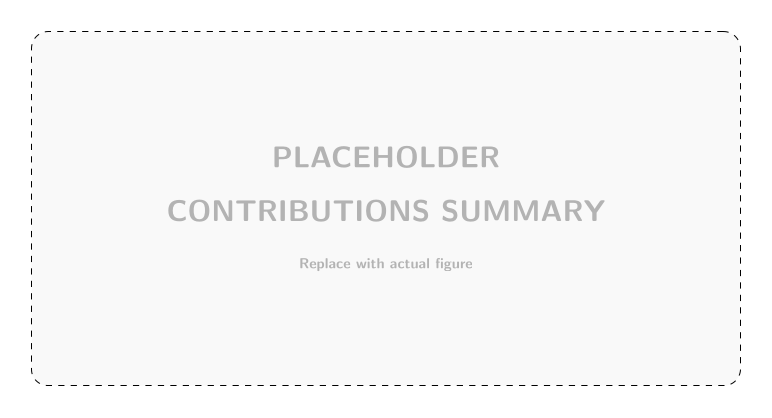
\includegraphics[width=0.85\textwidth]{Images/fig_contributions_summary.png}
\caption{Summary of project contributions mapped to the challenges they address in the e-voting landscape.}
\label{fig:contributions}
\end{figure}

\section{Achievement Against Objectives}

\begin{table}[H]
\centering
\caption{Evaluation of achievement against stated project objectives.}
\label{tab:objectives-eval}
\resizebox{\textwidth}{!}{%
\begin{tabular}{|c|p{5cm}|l|p{5cm}|}
\hline
\textbf{\#} & \textbf{Objective} & \textbf{Status} & \textbf{Evidence} \\
\hline
1 & Design ZK circuit proving voter membership without revealing identity & Achieved & Noir circuit with 4 constraints; UltraHonk proof verified on-chain \\
\hline
2 & Develop smart contracts with five layers of fraud prevention & Achieved & Voting.sol, ElectionRegistry, NicRegistry, HonkVerifier deployed and tested \\
\hline
3 & Build a custom gasless blockchain embedding the EVM & Achieved & Go blockchain with BoltDB, PBFT, REST API; executes same bytecode as Hardhat \\
\hline
4 & Develop mobile app with hardware security and on-device proving & Achieved & React Native (Expo 54); expo-secure-store; WebView bb.js WASM proving \\
\hline
5 & Implement web administration for EA and GN officers & Achieved & Next.js app with admin dashboard, GN portal, results page \\
\hline
6 & Model 160-division structure with national aggregation & Achieved & ElectionRegistry factory; \texttt{getNationalResults()} aggregation \\
\hline
7 & Achieve formal voter--ballot unlinkability & Achieved & Theorem~\ref{thm:unlinkability}: $\Pr[\mathcal{A} \to (\text{V}, \text{B})] \leq 1/|\mathcal{V}| + \text{negl}(\lambda)$ \\
\hline
\end{tabular}%
}
\end{table}

All seven project objectives have been achieved. The system demonstrates a complete, working prototype of a privacy-preserving electronic voting system with mathematical security guarantees.

\section{Limitations}

We acknowledge the following limitations of the current implementation:

\subsection{Ballot Secrecy}

Our system provides \textit{voter--ballot unlinkability} (no one can determine who cast which ballot) but not full \textit{ballot secrecy} (individual vote values are visible on-chain after counting). True ballot secrecy requires homomorphic tallying, where votes are encrypted and the tally is computed on ciphertexts without decrypting individual ballots. This is a fundamental limitation addressed in future work.

\subsection{Coercion Resistance}

While the burner wallet mechanism prevents post-hoc proof of vote, a physically present coercer can observe the voting screen in real-time. Full coercion resistance requires the ability to re-vote secretly (as in MACI) or deniable encryption schemes.

\subsection{Proof Generation Time}

The 15--25 second proof generation time on mobile, while acceptable for a once-per-election action, falls below the $<$5 second threshold expected for consumer applications. This is an engineering limitation (WASM execution in WebView) rather than a fundamental one.

\subsection{Trusted Ceremony for SRS}

While UltraHonk eliminates per-circuit trusted setup, it still uses a universal Structured Reference String (SRS) from the Aztec Ignition ceremony. In theory, if all ceremony participants collude, the soundness guarantee could be broken. In practice, the ceremony involved thousands of participants, making collusion computationally infeasible.

\subsection{Mobile Platform Limitations}

\begin{itemize}
    \item \textbf{iOS}: Face ID integration requires a custom development build (\texttt{NSFaceIDUsageDescription}); not tested in Expo Go
    \item \textbf{Root/jailbreak}: No detection implemented; a rooted device could potentially extract keystore secrets
    \item \textbf{Hermes BigInt}: The workaround (WebView proving) adds architectural complexity
\end{itemize}

\subsection{Production Readiness}

The system is a research prototype, not production-ready software. Gaps include:
\begin{itemize}
    \item No formal security audit by third-party experts
    \item No stress testing at 16M voter scale
    \item Development OTP provider (not production SMS gateway)
    \item No CI/CD pipeline or monitoring infrastructure
    \item No accessibility features (screen reader, high contrast, multi-language)
\end{itemize}

\section{Future Work}

\begin{figure}[H]
\centering
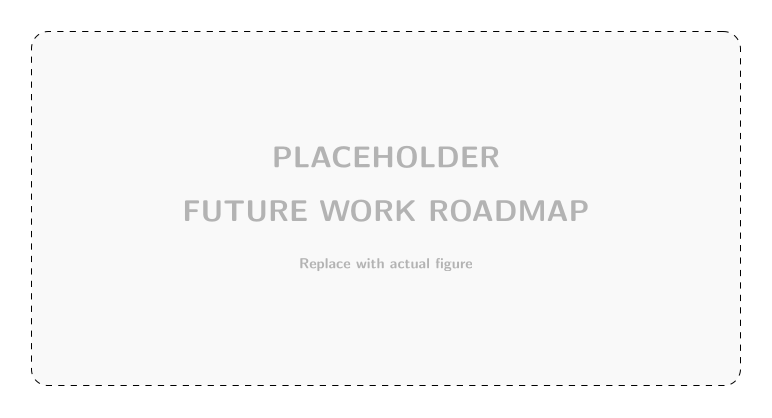
\includegraphics[width=0.85\textwidth]{Images/fig_future_work_roadmap.png}
\caption{Future work roadmap: short-term engineering improvements, medium-term protocol upgrades, and long-term research directions.}
\label{fig:future-roadmap}
\end{figure}

\subsection{Short-Term: Engineering Improvements}

\begin{enumerate}
    \item \textbf{Native ZK Proving}: Integrate Swoir (Noir's native mobile prover) or noir\_android to reduce proof generation from 15--25 seconds to $<$5 seconds. This eliminates the WebView architecture entirely.
    
    \item \textbf{Production OTP}: Replace the development OTP system with Firebase Authentication or Twilio for production-grade SMS verification with rate limiting and fraud detection.
    
    \item \textbf{ERC-4337 Paymaster}: For L2 deployment scenarios, implement an account abstraction paymaster that sponsors burner wallet gas fees without requiring a custom chain.
    
    \item \textbf{Root/Jailbreak Detection}: Integrate SafetyNet (Android) and App Attest (iOS) to prevent voting from compromised devices where keystore security guarantees are voided.
\end{enumerate}

\subsection{Medium-Term: Protocol Upgrades}

\begin{enumerate}
    \item \textbf{Homomorphic Tallying}: Implement additively homomorphic encryption (e.g., exponential ElGamal) where:
    \begin{equation}
    \text{Tally} = \text{Dec}\left(\prod_{i=1}^{n} \text{Enc}(v_i)\right) = \sum_{i=1}^{n} v_i
    \end{equation}
    This achieves full ballot secrecy---no entity ever sees individual decrypted votes. The tally is decrypted only in aggregate via threshold decryption among election commission nodes.
    
    \item \textbf{Re-Voting for Coercion Resistance}: Allow voters to submit multiple ballots (only the last counts), with the re-voting action hidden from observers. This requires encrypted ballot storage and a trusted coordinator to process the override logic---a trade-off between coercion resistance and trust minimization.
    
    \item \textbf{Formal Verification}: Verify the Noir circuit using automated theorem provers (Lean 4, Z3) to mathematically prove that:
    \begin{itemize}
        \item No valid proof can be generated without a valid witness
        \item The circuit faithfully implements the specified security properties
        \item No constraint under-specification allows exploits
    \end{itemize}
\end{enumerate}

\subsection{Long-Term: Research Directions}

\begin{enumerate}
    \item \textbf{Multi-Party Computation (MPC) Ceremony}: Conduct a public, verifiable MPC ceremony for the universal SRS, involving Sri Lankan institutions (universities, civil society, opposition parties) as participants. This provides transparent, auditable trust distribution.
    
    \item \textbf{Recursive Proofs for Scalability}: Use recursive proof composition (IVC/PCD) to aggregate thousands of individual vote proofs into a single proof, enabling $O(1)$ on-chain verification for the entire election:
    \begin{equation}
    \pi_{\text{aggregate}} = \text{Fold}(\pi_1, \pi_2, \ldots, \pi_n) \quad |\pi_{\text{aggregate}}| = O(1)
    \end{equation}
    
    \item \textbf{Post-Quantum Security}: Migrate from BN254 (vulnerable to quantum algorithms) to lattice-based proof systems (e.g., Plonky3 over Goldilocks field) that provide post-quantum security guarantees.
    
    \item \textbf{Decentralized Identity Integration}: Replace wallet-based voter identity with W3C Decentralized Identifiers (DIDs) and Verifiable Credentials, enabling interoperability with national digital identity systems.
    
    \item \textbf{Cross-Chain Interoperability}: Enable election result publication across multiple chains (Ethereum, Polygon, etc.) for maximum transparency and auditability by international observers.
\end{enumerate}

\section{Broader Impact}

This work demonstrates that the apparent conflict between voter privacy and election transparency can be resolved through modern cryptography. Zero-knowledge proofs enable a paradigm shift: from ``trust the authority'' to ``trust the mathematics.''

For Sri Lanka specifically, where election logistics cost millions of dollars and results take 24--48 hours to announce, a blockchain voting system could provide:
\begin{itemize}
    \item Instant results (tallies update in real-time)
    \item Zero logistical cost for ballot transport and counting
    \item Accessibility for overseas citizens and disabled voters
    \item Mathematical proof of election integrity (no recounts needed)
    \item Reduced human error in counting and tabulation
\end{itemize}

\section{Concluding Remarks}

We have presented a complete, working implementation of a privacy-preserving electronic voting system that combines zero-knowledge proofs, a custom blockchain, hardware-secured mobile authentication, and multi-division national architecture. Our system achieves formal voter--ballot unlinkability without requiring any trusted third party---a property that no prior deployed system has accomplished.

The journey from initial concept to working prototype involved four circuit iterations, three contract architecture generations, and numerous integration challenges (Poseidon field mismatches, Hermes BigInt limitations, EVM precompile registration). Each failure taught us something essential about the intersection of theoretical cryptography and practical engineering.

While significant work remains before production deployment---particularly homomorphic tallying, native proving, and formal verification---this project establishes that the fundamental architecture is sound and implementable with current technology. The combination of UltraHonk (no trusted setup), a custom gasless chain (economic inclusivity), and hardware-backed mobile security (physical presence verification) represents a viable path toward truly private, truly verifiable, and truly accessible democratic elections.

\vspace{1cm}

\begin{quote}
\textit{``The ballot is stronger than the bullet.''} --- Abraham Lincoln

\vspace{0.3cm}

We add: \textit{``And a zero-knowledge proof is stronger than both---for it proves truth without revealing secrets.''}
\end{quote}
